\chapter{Mass Exchange in Dead Water Zones: A Numerical Approach}
\label{chap:art1}
In this chapter, the first topic of the dissertation is presented as a published conference paper. The objective of this paper was to develop a simple numerical method capable of estimating the flow and the mass exchange between consecutive groyne fields and the main channel.

The original paper was published in the book 'Water, Energy and Food Nexus in the Context of Strategies for Climate Change Mitigation', under Spring publishing and can be found in \url{https://www.springer.com/gp/book/9783030572341}.
\section*{Authors}
\begin{itemize}
    \item Luiz Eduardo Domingos de Oliveira \footnote[1]{Federal University of Mato Grosso do Sul}
    \item Johannes Gérson Janzen \footnotemark[1]
\end{itemize}
\addcontentsline{toc}{section}{Abstract}
\section*{Abstract}
Dead water zones (DWZs) in natural open channels, formed by consecutive groynes, are regions separated from the main channel, characterized by recirculating flows. These regions present smaller velocities compared to the main channel, increasing the deposition of sediment and the temporary storage of polluted materials. Exchange processes between DWZs and the main channel influence the transport of pollutants in channels. This study adopts the k-omega shear stress transport (SST) turbulence model to examine the mass exchange between the main channel and the DWZ created by an infinite series of groynes. The computational results were compared to data collected in literature. A good agreement was achieved in mass exchange coefficient, with a relative error of approximately 2\%.

\noindent\textbf{Keywords:} Dead water zones (DWZ); Groyne Fields; Mass Exchange; Open Channel; Computational Fluid Dynamics (CFD).

\section{Introduction}
In fluvial engineering, channels are generally shaped by complicated boundaries that can be composed by dead water zones (DWZ), which can be formed by consecutive groynes \cite{xiang2019}. Groynes are transversal dykes placed in sequence along riverbanks keeping the flow away from the banks. The effects of this structure in rivers are an increase in mean velocity and water depth in the main channel, improved navigability; increased efficiency of sediment transport; protection against flooding and the mitigation of bank erosion \cite{mcCoy2008}. Its placement also provides lateral heterogeneity that can favour the presence of aquatic organisms, improving the biodiversity of river ecosystems \cite{mcCoy2008,Szlauer-ukaszewska2015,Buczynski2017,Mignot2017,Buczynska2018,xiang2019}.

Since the magnitude of mean flow velocities inside the DWZ is approximately 25\% of the flow velocities in the main channel, not only the deposition of sediment is enhanced, but also nutrients and contaminants which are readily attached to fine particles \cite{sukhodolov2014}. For instance, the attachment of contaminants to particles was observed in the Middle Elbe River, in Germany, leading to a low standard classification from an ecological view \cite{SchwartzKozerski2003}. The authors found, in the groyne fields, the deposition of fresh organic mud with high nutrient and pollution content (e.g. nitrogen). The deposition of pollution content attached to sediments creates a problem for river management \cite{uijttewaal2005}, especially in flood seasons, when the groyne field becomes submersed, being a source of contaminants to the main channel.

Therefore, in order to estimate the transport of pollutants in a channel, it is important to be able to understand and predict the exchange processes between the main channel and the DWZ formed between groynes \cite{weitbrecht2001}. These exchange processes were studied in detail in a series of laboratorial experiments carried out by \textcite{weitbrecht2004}. \textcite{Hinterberger2007} used large eddy simulation (LES) to model Weitbrecht’ experimental results. Although being a very precise model, LES is also more time consuming when compared to simpler models. Therefore, this study aims to investigate the mass exchange between the main channel and the groyne field using a simpler two-equations turbulence model, k-omega SST. The computational results are compared to Weibrecht results and a good agreement was obtained.

\section{Methods}
The geometry was chosen to match the groynes from the second series of experiments described in \textcite{weitbrecht2004}. The flow depth ($h$) was kept constant at 0.046 m and the experimental channel width ($B$) at 1.80m. The emergent groynes were 0.50m long ($W$) and spaced 1.25m apart ($L$), producing an aspect ratio of $W/L = 0.40$. The groyne heads were in a semi-circle format with diameter of 0.05m. The Reynolds number was 7360, and thereby turbulent.

The flow past the most downstream-located groyne in the series had a periodic behaviour \cite{Hinterberger2007}. Consequently, only one complete groyne field and two halves (located upstream and downstream from the complete one) was computed and a translational periodic boundary condition was imposed (Figure \ref{fig:art1:numericalDomainArticle1}). The mean streamwise velocity in the computational domain was approximately $U = 11 cm/s$, which corresponds to a mass flux of 6.56 kg/m² of water in the periodic zones. 

As the effects of the obstacles in the main channel extends up to one obstacle length in the transversal direction (y-axis) \cite{Brevis2014} the domain was two-thirds of the experimental flume width (B), reducing the computational effort. A free-slip symmetry boundary condition was imposed on the surface (Figure \ref{fig:art1:numericalDomainArticle1}). This boundary condition was also used on the free surface plane as it is an acceptable simplification for flows with Froude numbers smaller than 0.5 (our Froude number was 0.24) \cite{alfrink1983}. All walls, bed, lower side wall and groyne walls were considered hydraulically smooth.

\begin{figure}[!ht]
\centering
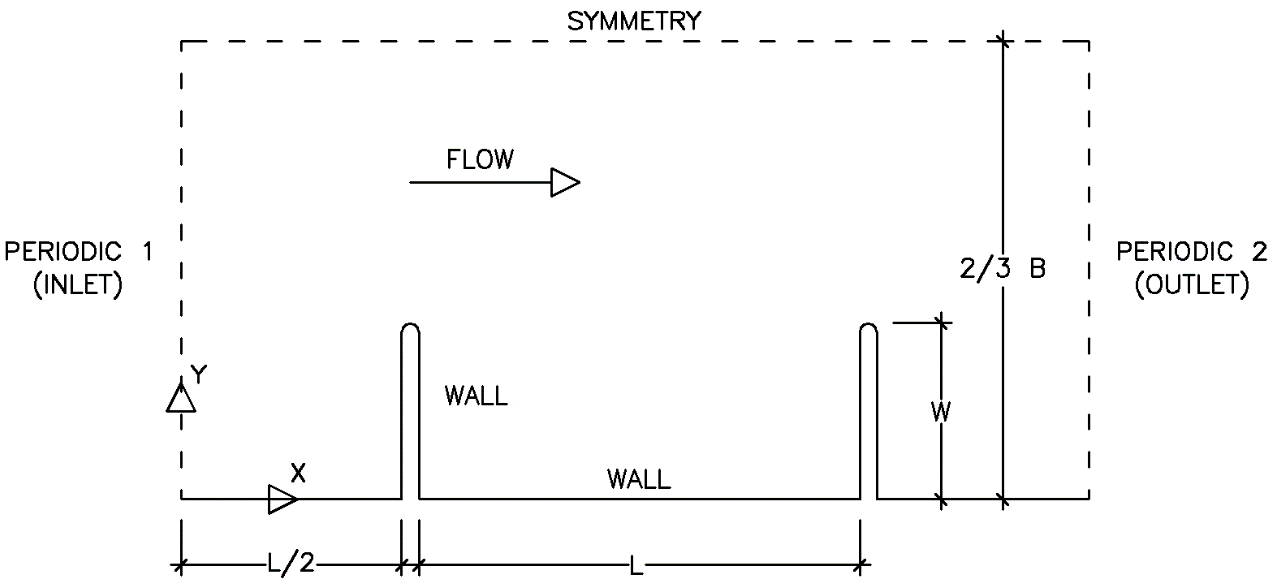
\includegraphics[width=\linewidth]{../images/art1/imgMassExchange1.png}
\caption{Upper view of the computational domain, from the free surface, and its boundary conditions.}
\label{fig:art1:numericalDomainArticle1}
\end{figure}

The domain was calculated in a three-dimensional grid (Figure \ref{fig:art1:mesh} a). The spatial discretization had a higher refinement in regions close to walls and at high velocity gradients regions. The meshing of the groyne’s heads considered its curvature and the proximity to the wall. This region used an O-grid with increasing element size (Figure \ref{fig:art1:mesh} b). The mesh had 20 divisions in the z-axis, increasing gradually from the bottom of the channel to its free surface (Figure \ref{fig:art1:mesh} c). In the y-axis, the groyne field had 70 divisions that gradually increased in size as it gets closer to the middle of the field. The strip that contains the groyne’s heads had finer elements due to the momentum transfer in the shear layer. The total grid presented approximately one million elements.

The commercial software called Ansys® FLUENT (version 14) was used to solve the grid, using the finite volume method to discretize the governing mass and momentum equations. The turbulent model chosen is based at Reynolds-averaged Navier-Stokes equations (RANS) approach, that consists of time averaged equations for fluid flow. The turbulent calculations were solved using the k-omega SST model proposed by \textcite{Menter2005}, due to its capability of solving fluid flow in low Reynolds numbers. The pressure-velocity coupling method was SIMPLE and the gradient spatial discretization was Least Squares Cell Based. The momentum was discretized in a third order MUSCL scheme. The turbulent kinect energy ($tke$) and specific dissipation rate ($\omega$) were discretized in a second order upwind scheme.

In addition to the velocity field, tracer concentration fields were also calculated by solving the following transport equation 
\begin{equation}
\frac{\partial}{\partial t}(\rho Y_i)+\nabla (\rho \vec{v} Y_i)=\nabla (\rho D_{i,m}+\frac{\mu_t}{Sc_t})\nabla Y_i
\label{eqn:art1:transportEq}
\end{equation}\begin{equation}
Sc_t = \frac{\mu_t}{\rho D_t}
\label{eqn:art1:Sct}
\end{equation}
where $\rho$ is the fluid mass density, $Y_i$ is the local mass fraction of each species, $D_{i,m}$ is the mass diffusion coefficient for species in the mixture, $\vec{v}$ is the velocity vector, $Sc_t$ is the turbulent Schmidt number (Equation \ref{eqn:art1:Sct}), $\mu_t$ turbulent viscosity and $D_t$ the turbulent diffusivity. In other terms, the transport equation means that the rate of change and the net rate of flow (convection) equals the rate of change due to diffusion.

Equation (\ref{eqn:art1:transportEq}) does not consider any chemical reactions or addition of phases during the solution and was discretized in a second order upwind scheme. The tracer was conservative, pursuing the same properties than water.

\begin{figure}[!ht]
\centering
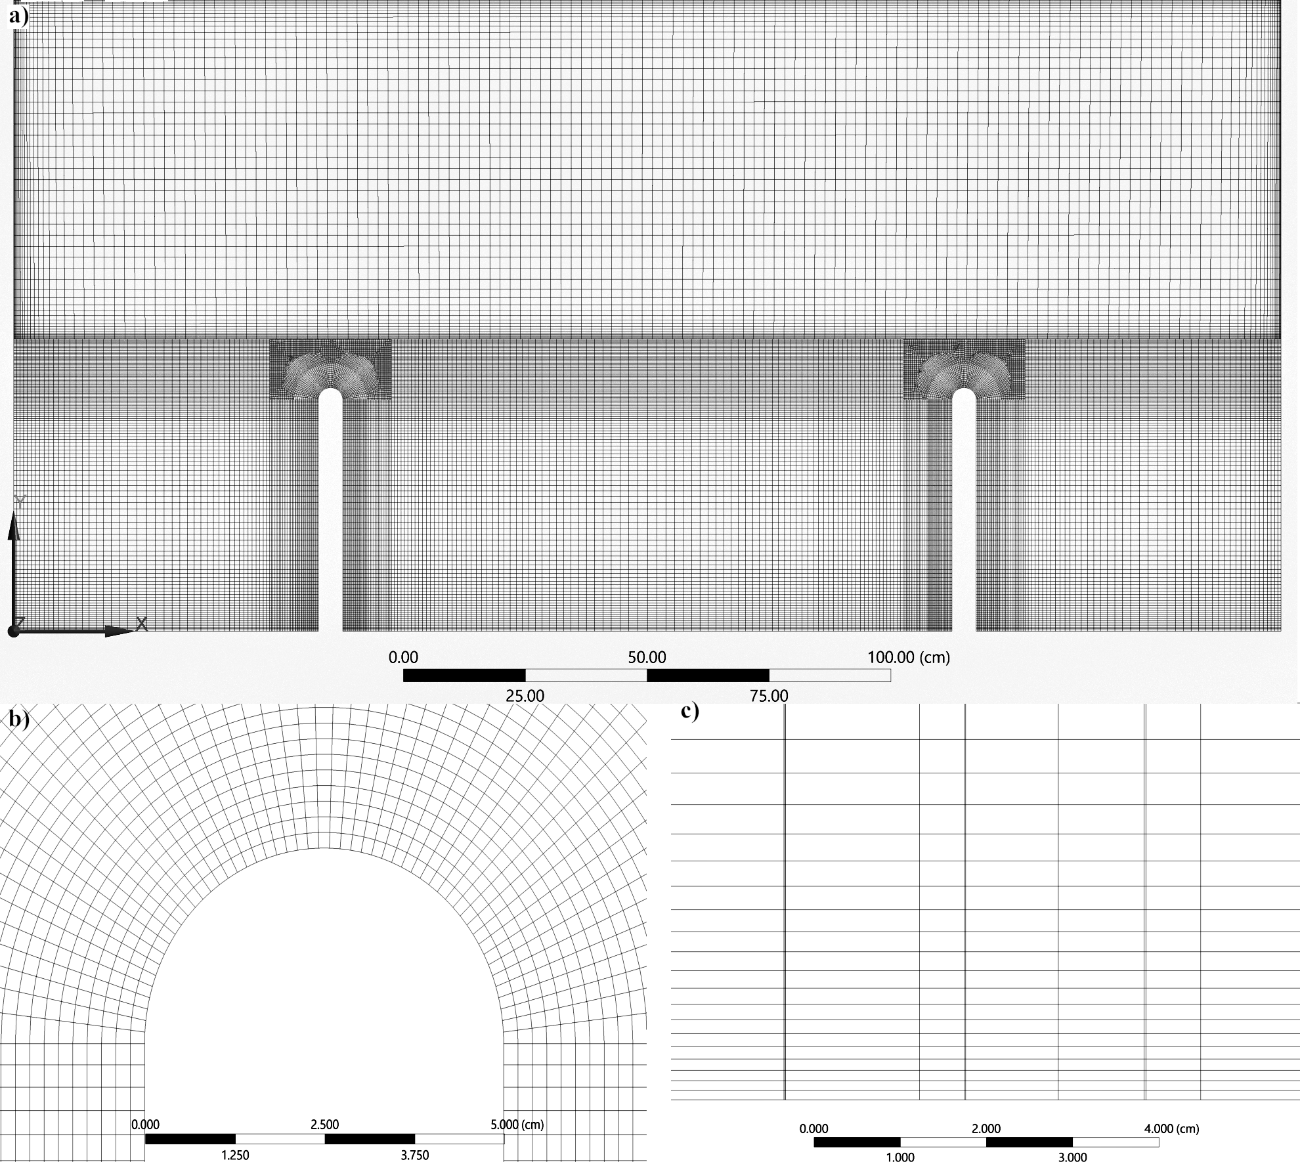
\includegraphics[width=\linewidth]{../images/art1/imgMassExchange2.png}
\caption{Computational mesh: a) mesh in the free-surface plane; b) curvilinear grid around groyne tip; c) mesh in a vertical plane near the middle of the groyne field.}
\label{fig:art1:mesh}
\end{figure}

The time step in the simulation was $0.024h/U$. The simulation was run for nearly $180h/U$ until the fully developed state was achieved. Once the flow reached the fully developed state, the tracer mass fraction was set to 1 within the groyne field and 0 in the other parts of the channel. Then, statistics of the mean flow and tracer transport were calculated using the instantaneous flow fields and mean tracer concentration inside the groyne field over the next $548h/U$.

\section{Results and Discussion}
Two gyres could be observed in the groyne field. A large primary gyre (right vortex in the central groyne field) and a small secondary gyre in the upstream groyne (Figure \ref{fig:art1:contour}). The formation of this system occurred by the momentum transferred by the main channel through a mixing layer. As the main flow went downstream, the shear in between zones excited an anticlockwise gyre (primary gyre) that further excited a smaller clockwise circulation (secondary gyre) that had no contact with the main channel. The secondary gyre was smaller in size (approximately 21\% of the groyne field area) and velocity magnitudes, when compared to the mean circulation (Figure \ref{fig:art1:contour}).

\begin{figure}[!ht]
\centering
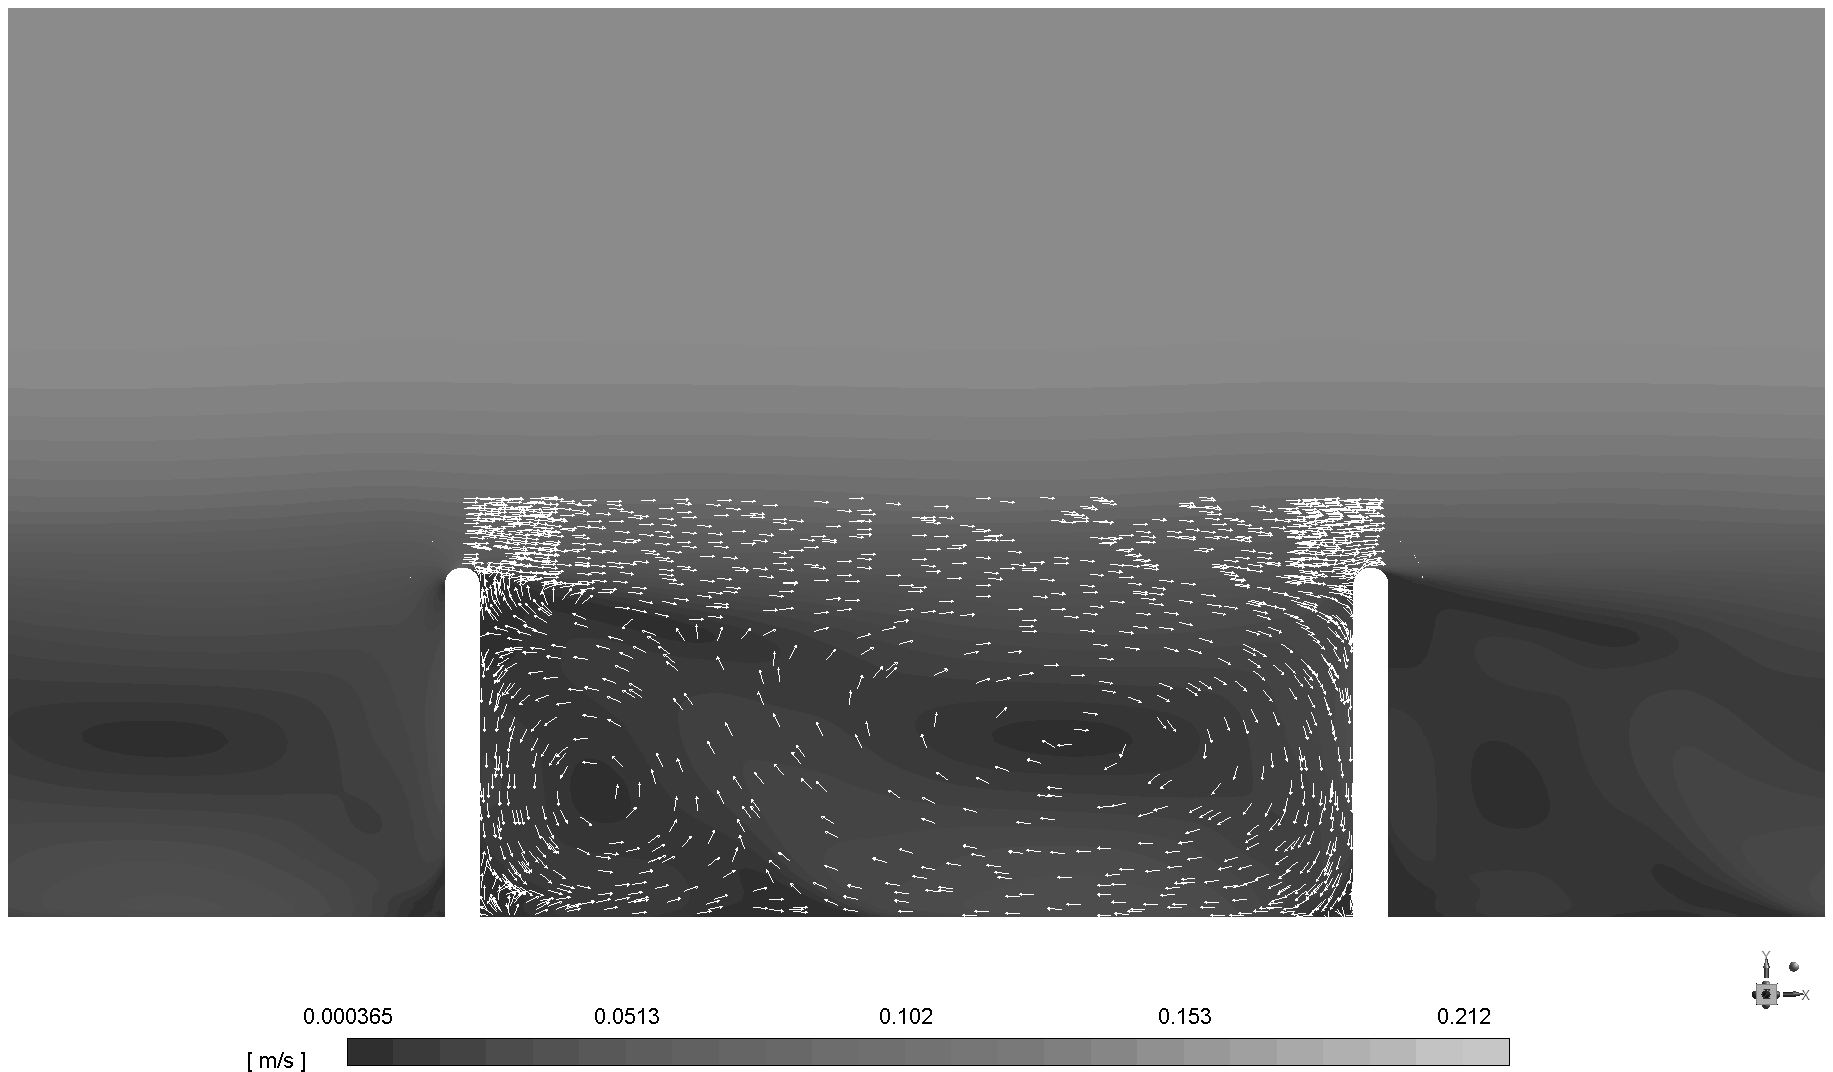
\includegraphics[width=\linewidth]{../images/art1/imgMassExchange3.png}
\caption{Mean velocity contour.}
\label{fig:art1:contour}
\end{figure}

Figure \ref{fig:art1:graphs} shows the mean streamwise velocity distributions for x/L = 0.25, 0.50 and 0.75 (x has origin in the right face of the first groyne and points to the right). Overall, the model had a good accordance in the main channel and in the central part of the groyne field. The computational model was able to capture the circulation pattern inside the groyne field. However, near the groyne heads (interface between the main channel and the groyne fields) the concordance was not so good. This is due to the high dissipation of momentum that occurred in the mixing layer. Despite the fine resolution of the grid, the model could not describe the flow inside this region. For the same reason the secondary gyre did not have contact with the mixing layer, since this vortex was formed by the dissipation of momentum from the primary gyre. The mean error was approximately 102\%, 21 \% and 47 \% for Figure \ref{fig:art1:graphs} a), b) and c), respectively. However, the flow was in the same order of magnitude than the experimental, which indicates that (Figure \ref{fig:art1:contour}) represents qualitatively, at least, the flow within the region.

The ejection of tracer from a groyne field to the mixing layer (region between the DWZ and the main channel) occurs in the upstream portion of the field (up to 40\%), while the following 60\% is a region where mass can re-enter the system \cite{weitbrecht2004}. The tracer concentration stayed higher in the secondary gyre, while the primary gyre oscillated due to the injection of tracer from the mixing layer and its natural ejection (Figure \ref{fig:art1:tracerContour}). This movement was captured by the model and can be seen completely in https://youtu.be/9b-4JZJdeA0.

\begin{figure}[!ht]
\centering
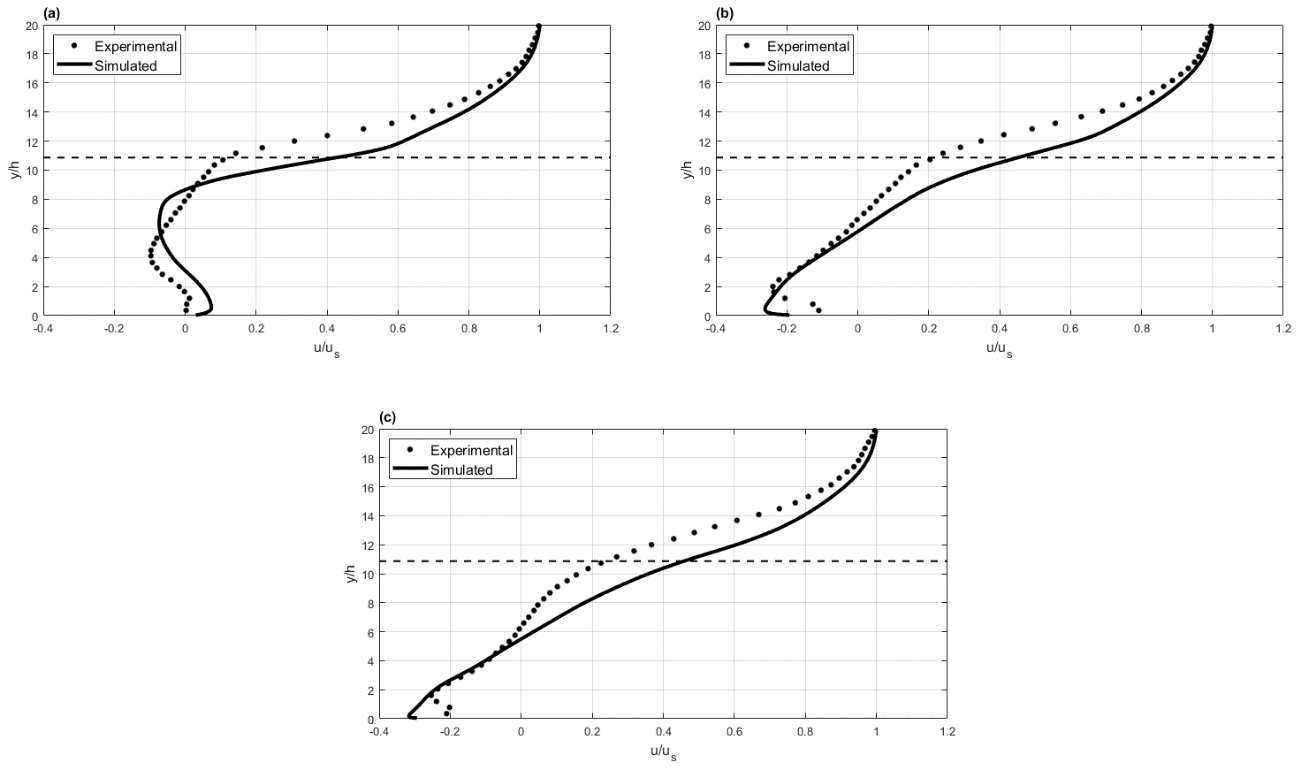
\includegraphics[width=\linewidth]{../images/art1/imgMassExchange4.png}
\caption{Mean streamwise velocity distributions. a) x/L = 0.25 b) x/L = 0.50 and c) x/L = 0.75. The dashed line represents the groyne head position (y/h = 10.87).}
\label{fig:art1:graphs}
\end{figure}
\begin{figure}[!ht]
\centering
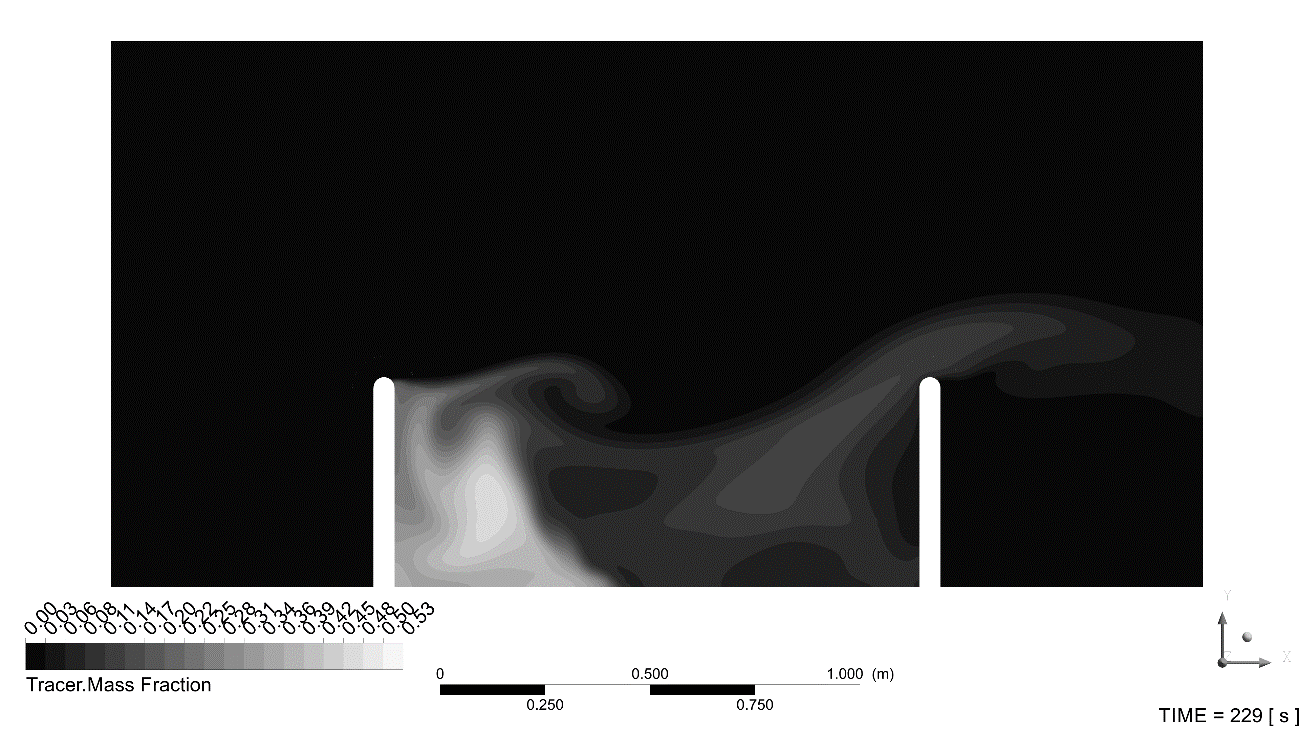
\includegraphics[width=\linewidth]{../images/art1/imgMassExchange5.png}
\caption{Tracer mass fraction in the free-surface plane in time 229s.}
\label{fig:art1:tracerContour}
\end{figure}

The tracer concentration inside the field was fitted in a first order decay model (Equation \ref{eqn:art1:massDecay}) following the same procedure from the experimental study (Figure \ref{fig:art1:massGraph1}).
\begin{equation}
C=C_0 e^{\frac{-t}{MRT}}
\label{eqn:art1:massDecay}
\end{equation}
Where MRT is the mean retention time. Based on the MRT, the mass coefficient k (Equation \ref{eqn:art1:k}) was calculated in order to estimate the intensity of mass exchange \cite{weitbrecht2001}.
\begin{equation}
k=\frac{W}{MRT U}
\label{eqn:art1:k}
\end{equation}The fitted curve presented an $MRT = 117.7s$ that related to an exchange coefficient of $k = 0.026$. The relative error between the mean value of Weitbrecht’ experiments and our model was 1.99\% for the exchange coefficient and 1.69 \% for MRT (Table \ref{tab:art1:kVal}).

Although we could observe a good fitting between our computational model and the experimental results, it can be observed that the system presented two slopes, with a breakpoint near $C/C0 = 0.2$ (Figure \ref{fig:art1:massGraph1}). The first slope was influenced by the tracer concentration present in the primary gyre, that oscillates between ejecting mass and re-absorbing via the shear layer. The second one ejects mass slower, as the concentration in the field was mainly disposed in the secondary gyre. Figure \ref{fig:art1:massGraph2} shows the tracer concentration fitted in two curves, the first curve presented an $MRT = 113.27s$ and a $k = 0.0274$ while the second $MRT = 121.43s$ and $k = 0.0256$. The summary of the model and comparisons with previous studies can be seen in Table \ref{tab:art1:kVal}.

Our results are consistent with field observations. \textcite{sukhodolov2014}, for example, observed that the mass concentrated in the secondary gyre, since it presented the slowest velocities in the groyne field.

\begin{figure}[!ht]
\centering
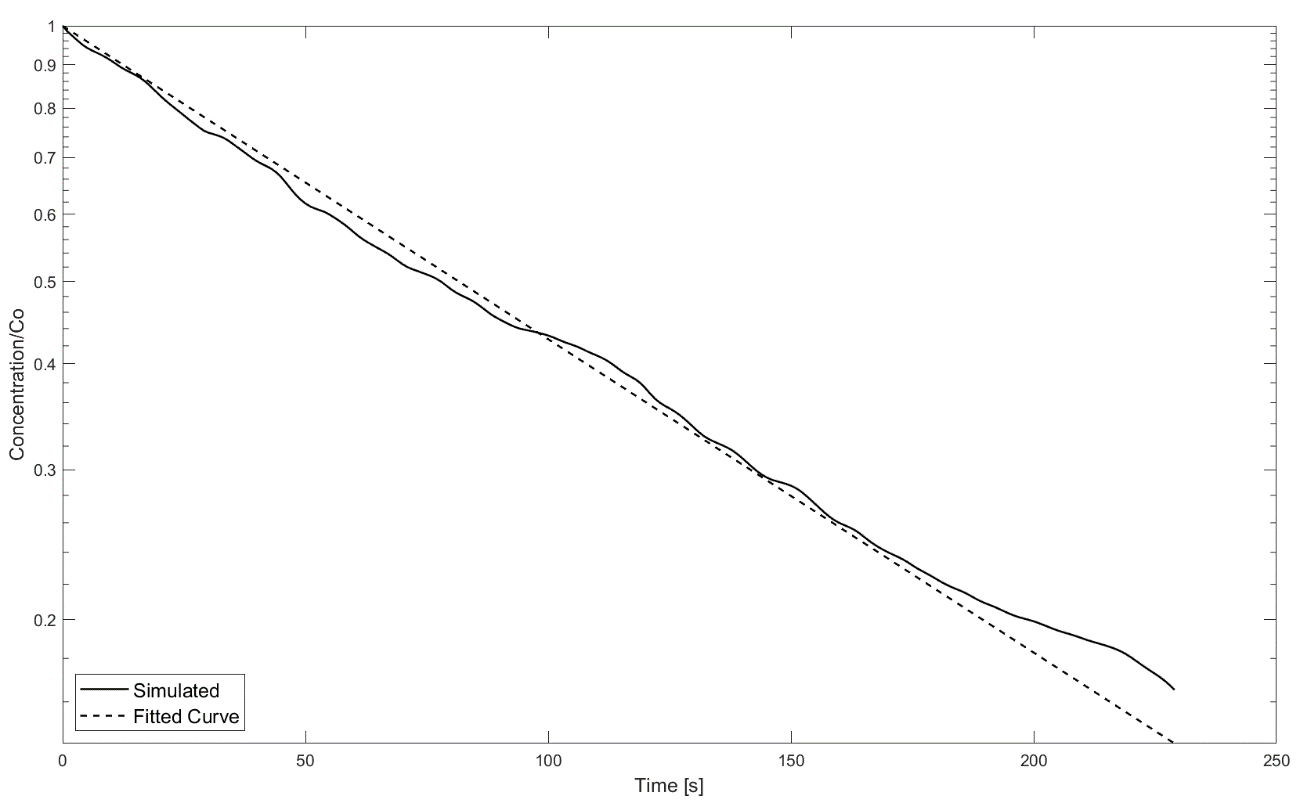
\includegraphics[width=\linewidth]{../images/art1/imgMassExchange6.png}
\caption{Volumetric averaged mass concentration inside groyne field.}
\label{fig:art1:massGraph1}
\end{figure}
\begin{figure}[!ht]
\centering
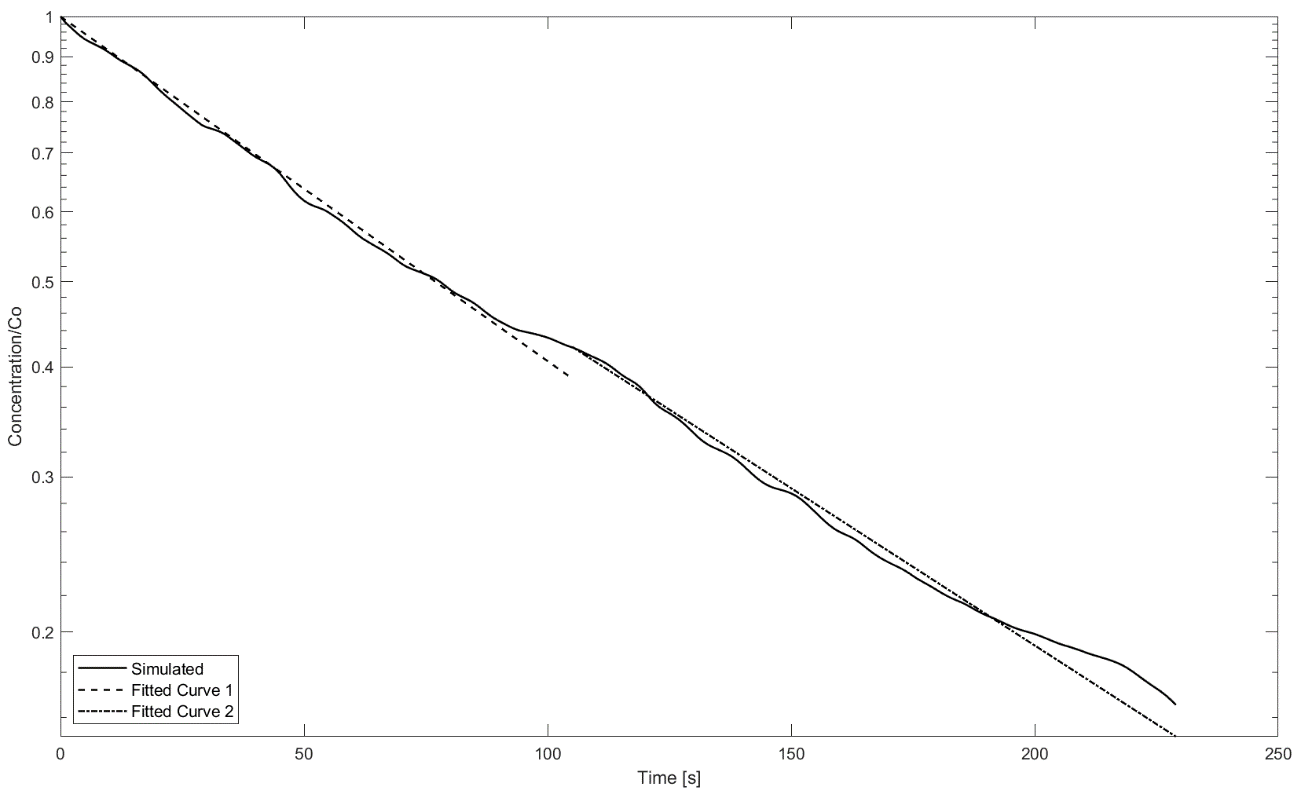
\includegraphics[width=\linewidth]{../images/art1/imgMassExchange7.png}
\caption{Volumetric averaged mass concentration inside groyne field fitted with two curves.}
\label{fig:art1:massGraph2}
\end{figure}
\begin{table}[]
\centering
\caption{Comparison of mean residence time inside groyne field and exchange coefficient in between experimental and numerical studies.}
\label{tab:art1:kVal}
\begin{tabular}{lll}
Experiment/Model                     & MRT {[}s{]} & k      \\ \hline
Experiment 1                         & 97          & 0.029  \\
Experiment 2                         & 114         & 0.028  \\
Experiment 3                         & 125         & 0.022  \\
Mean value of experiments            & 118         & 0.027  \\
3D LES \textbackslash{}cite\{Hinterberger2007\}                                            & 137 & 0.023 \\
\begin{tabular}[c]{@{}l@{}}2D LES \textbackslash{}cite\{\\ Hinterberger2007\}\end{tabular} & 75  & 0.042 \\
3D k-omega SST (global fitted curve) & 117.7       & 0.026  \\
3D k-omega SST (first slope)         & 113.3       & 0.0274 \\
3D k-omega SST (second slope)        & 121.62      & 0.0256 \\ \hline
\end{tabular}
\end{table}

\section{Conclusion}
A 3D k-omega SST simulation was presented for a periodic shallow water flow in a groyne field. Out model was able to reproduce a similar structure and magnitude flow compared to experimental data. Furthermore, our model could predict the mass exchange coefficient between the main channel and the DWZ and the mean retention time of the DWZ, being in good concordance with experimental results. In agreement to experimental and field observations, the decay of mass inside the field is described in two phases, first when the primary gyre dominates the ejection and second when the mass in concentrated in the second gyre prolonging the MRT. Hence, a simpler model than LES can predict the main parameters related to the mass exchange process in groyne structures.

%\nomenclature{$h$}{Flow Depth\nomunit{$m$}}
%\nomenclature{$B$}{Experimental channel width\nomunit{$m$}}
%\nomenclature{$W$}{Groyne field width\nomunit{$m$}}
%\nomenclature{$L$}{Groyne field length\nomunit{$m$}}
%\nomenclature{$U$}{Mean streamwise velocity in the main channel\nomunit{$m/s$}}
%\nomenclature{$tke$}{Turbulent kinetic energy\nomunit{$m^2/s^2$}}
%\nomenclature{$\omega$}{Specific dissipation rate\nomunit{$1/s$}}
%\nomenclature{$\rho$}{Fluid mass density\nomunit{$kg/m^3$}}
%\nomenclature{$Y_i$}{Local mass fraction of each species}
%\nomenclature{$D_{i,m}$}{Mass diffusion coefficient for the species in the mixture}
%\nomenclature{$\vec{v}$}{Velocity vector\nomunit{$m/s$}}
%\nomenclature{$Sc_t$}{Turbulent Schmidt number}
%\nomenclature{$\mu_t$}{Turbulent viscosity\nomunit{$kg/m s$}}
%\nomenclature{$D_t$}{Turbulent diffusivity\nomunit{$m^2/s$}}
%\nomenclature{$C$}{Concentration}
%\nomenclature{$MRT$}{Mean retention time\nomunit{$s$}}
%\nomenclature{$t$}{Time\nomunit{$s$}}
%\nomenclature{$k$}{Mass exchange coefficient}
%\printnomenclature

\addcontentsline{toc}{section}{Acknowledgements}
\section*{Acknowledgements}
The authors are grateful to members of SCF laboratory for providing the necessary hardware. Specially, D.F. Silva, M.L.M. Xavier, P.H.S de Lima, T.C.R Ventura and T.N. Yamasaki for research assistance and hardware set up.

\addcontentsline{toc}{section}{Funding}
\section*{Funding}
This study was financed in part by the Coordenação de Aperfeiçoamento de Pessoal de Nível Superior - Brazil (CAPES) -Finance Code 001.
\addcontentsline{toc}{section}{References}
\printbibliography[segment=\therefsegment,heading=subbibliography, title={References}]